%----------- File: Kapitel/datenbank.tex -----------

\chapter{Datenbank}
\label{chap:datenbank}
\authormargin{Yolanda Hadiana Fiska}

%%%%%%%%%%%%%% Einleitung %%%%%%%%%%%%%%%%%%%%%%%%%%
Die Integration einer Datenbank stellt einen zentralen Bestandteil der Gesamtlösung dar.
Sie bildet die Grundlage für eine effiziente Speicherung, Verwaltung und spätere Analyse
der im Projekt erzeugten Transkriptionsdaten.

\section{Einleitung}
\label{sec:einleitung}
\authormargin{Yolanda Hadiana Fiska}

Die Nutzung einer durchsuchbaren Datenbank ist notwendig, da Meetings und Konferenzen
oft eine hohe Informationsdichte aufweisen. Ohne eine strukturierte Ablage wäre es für
Teilnehmer nahezu unmöglich, spezifische Aussagen oder Diskussionen effizient
wiederzufinden. Eine durchsuchbare Datenbank ermöglicht daher nicht nur die
automatisierte Dokumentation, sondern auch eine signifikante Verbesserung
der Nachverfolgbarkeit und Wissenssicherung.

Für die Datenbankintegration ergeben sich folgende zentrale Anforderungen:

\begin{itemize}
    \item \textbf{Speicherung:} Persistente Ablage der Transkripte in einer konsistenten Datenstruktur, die Metadaten zu Meetings und Sprechern einschließt.
    \item \textbf{Durchsuchbarkeit:} Unterstützung effizienter Volltextsuche mit sprachspezifischer Tokenisierung, Normalisierung und optionaler Fuzzy-Suche.
    \item \textbf{Skalierbarkeit:} Möglichkeit, auch große Datenmengen aus zahlreichen Meetings performant zu verwalten.
    \item \textbf{Echtzeit-Zugriff:} Sofortige Verfügbarkeit neu erfasster Transkriptionssegmente für nachfolgende Suche und Analyse.
\end{itemize}

Das primäre Ziel der Datenbankintegration besteht in der
\textbf{Ermöglichung einer strukturierten Ablage und einer effizienten Suche}
innerhalb von Transkripten. Damit wird die Grundlage geschaffen,
um Inhalte nicht nur zu dokumentieren, sondern sie auch als
nachhaltige Wissensbasis für Teilnehmer und Organisationen nutzbar zu machen.


%%%%%%%%%%%%% Datenmodellierung %%%%%%%%%%%%%%%%%%%%%%%
\section{Datenmodellierung}
\authormargin{Yolanda Hadiana Fiska}

Die Datenbankstruktur ist so gestaltet, dass sie sowohl die Speicherung der
Transkripte als auch deren effiziente Durchsuchbarkeit und Kontextualisierung ermöglicht.
Im Zentrum stehen drei Haupttabellen, deren Beziehungen im folgenden erläutert werden.

\subsection{Wichtige Tabellen}
\label{sec:datenmodell:tabellen}
\authormargin{Yolanda Hadiana Fiska}

\begin{itemize}
    \item \textbf{Besprechungen (\texttt{besprechungen}):}
    Enthält Metadaten zu einzelnen Meetings. Dazu gehören eine eindeutige ID, der Titel der Besprechung sowie das Erstellungsdatum.
    Diese Tabelle dient als Ankerpunkt für alle weiteren Informationen.

    \item \textbf{Sprecher (\texttt{sprecher}):}
    Speichert die Namen der an Meetings beteiligten Sprecher.
    Über das Fremdschlüsselfeld \texttt{besprechungen\_id} wird eine direkte Beziehung zur jeweiligen Besprechung hergestellt.

    \item \textbf{Aussagen (\texttt{aussagen}):}
    Enthält die eigentlichen Transkriptionsabschnitte. Neben den Roh- und verarbeiteten Texten
    werden hier Start- und Endzeitstempel, optionale Schlagwörter (\texttt{tags}),
    sowie ein generierter \texttt{tsvector} für die Volltextsuche abgelegt.
    Über Fremdschlüssel zu \texttt{sprecher} und \texttt{besprechungen}
    sind die Aussagen eindeutig einem Sprecher und einer Besprechung zugeordnet.
\end{itemize}

\subsection{Beziehungen zwischen den Tabellen}
\label{sec:datenmodell:relationen}
\authormargin{Yolanda Hadiana Fiska}

Zwischen den Tabellen bestehen folgende Beziehungen:

\begin{itemize}
    \item \textbf{1:n Beziehung zwischen \texttt{besprechungen} und \texttt{sprecher}:}
    Eine Besprechung kann mehrere Sprecher enthalten, ein Sprecher ist jedoch genau einer Besprechung zugeordnet.

    \item \textbf{1:n Beziehung zwischen \texttt{besprechungen} und \texttt{aussagen}:}
    Jede Besprechung kann mehrere Aussagen beinhalten.

    \item \textbf{1:n Beziehung zwischen \texttt{sprecher} und \texttt{aussagen}:}
    Ein Sprecher kann im Verlauf einer Besprechung mehrere Aussagen tätigen.
\end{itemize}

\subsection{Visualisierung}
\label{sec:datenmodell:visualisierung}
\authormargin{Yolanda Hadiana Fiska}

Das folgende ER-Diagramm veranschaulicht die Relationen zwischen den Tabellen:

\clearpage 
\begin{figure}[h!]
    \centering
    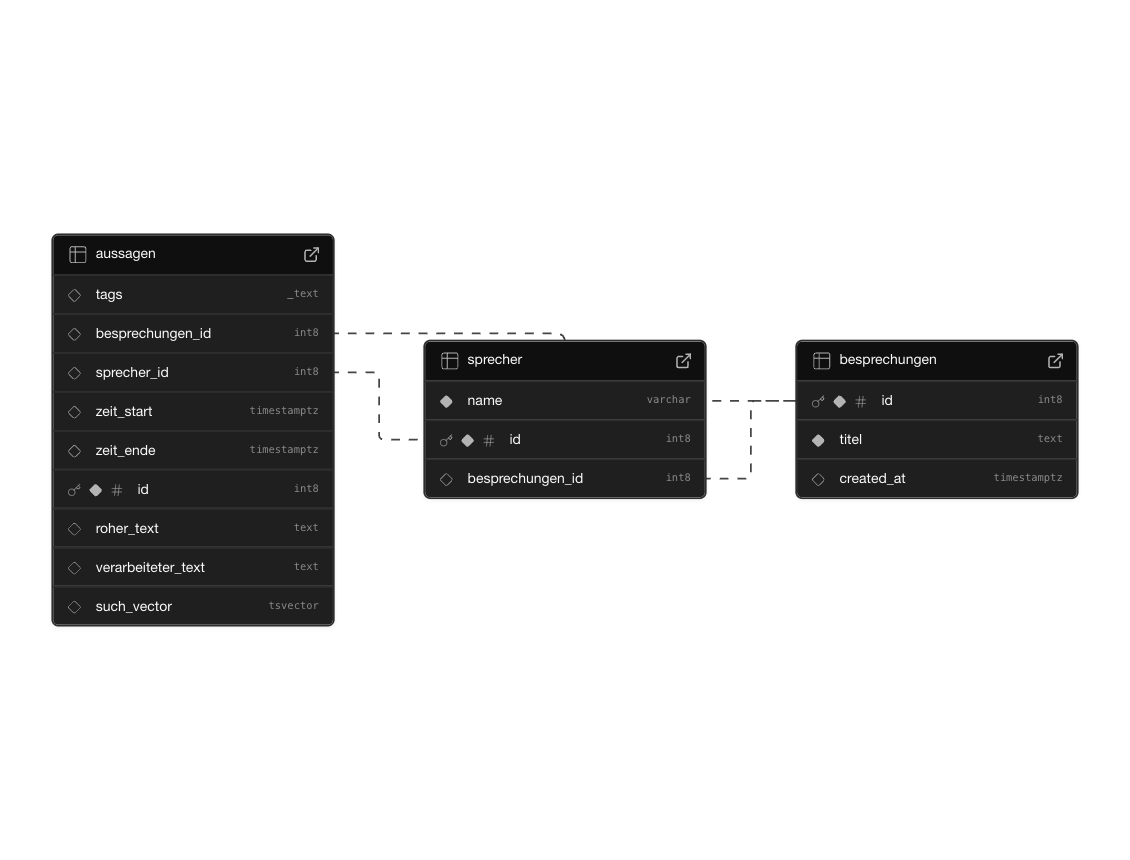
\includegraphics[width=0.9\textwidth]{Bilder/ERDiagram.png}
    \caption{ER-Diagramm der Datenbankstruktur (vereinfachte Darstellung)}
    \label{fig:er-diagramm}
\end{figure}


%%%%%%%%%% %%%% Technik- und Toolauswahl %%%%%%%%%%%%%%%%%%%
\section{Technik- und Toolauswahl}
\label{sec: toolauswahl}
\authormargin{Yolanda Hadiana Fiska}
Die Wahl geeigneter Technologien und Werkzeuge bildet eine zentrale Grundlage
für die erfolgreiche Umsetzung des Projekts. Neben fachlichen Anforderungen
wie Datenstruktur, Skalierbarkeit und Performance spielen auch praktische
Aspekte wie Wartbarkeit, Community-Support und Kompatibilität mit der
bestehenden Infrastruktur eine wichtige Rolle. In diesem Abschnitt werden die
getroffenen Entscheidungen zur Auswahl von Datenbanktechnologien und weiteren
Hilfsmitteln erläutert und begründet.

\subsection{Auswahl der Datenbanktechnologie}
\label{sec:loesung:db_auswahl}
\authormargin{Yolanda Hadiana Fiska}
Da die  Anwendung auf textbasierte Datenverarbeitung und insbesondere
auf performante Volltextsuche ausgelegt ist, stellt die Wahl der
Datenbanktechnologie einen entscheidenden Faktor dar. Verschiedene Optionen
wie relationale Datenbanken, dokumentenorientierte Systeme oder spezialisierte
Suchmaschinen wurden geprüft und hinsichtlich ihrer Eignung bewertet.

Nach einer Evaluierung verschiedener Technologien fiel die Wahl auf \textbf{Supabase}. Supabase ist eine Open-Source Backend-as-a-Service (BaaS) Plattform, die Entwicklern ermöglicht, moderne Web- und Mobile-Anwendungen zu erstellen, ohne sich um die komplexe Einrichtung eines eigenen Backends kümmern zu müssen \cite{supabaseLeWagon2025}. Die Plattform basiert auf \textbf{PostgreSQL} und bietet eine Vielzahl integrierter Werkzeuge, die speziell für die Anforderungen dieses Projekts geeignet sind – darunter moderne Schnittstellen, Echtzeit-Funktionalitäten und eingebaute Benutzer-Authentifizierung \cite{supabaseDocs2025}.

\subsection{Techniken und Tools für die Datenbankintegration:}
\authormargin{Yolanda Hadiana Fiska}
\begin{itemize}
  \item \textbf{PostgreSQL}: Relationale Datenbank mit hoher Zuverlässigkeit, Erweiterbarkeit und nativer Volltextsuche (\texttt{tsvector} + GIN-Index).
  \item \textbf{Qt-SQL-Schnittstelle}: Direkter Zugriff auf Supabase-Datenbank über standardisierte SQL-Verbindungen, ermöglicht Abfragen, Einfügungen und Updates.
  \item \textbf{\ac{RLS}}: Fein granulierte Zugriffskontrolle direkt auf Datenbankebene.
  \item \textbf{Realtime Engine}: WebSocket-basierte Echtzeit-Updates bei Datenänderungen, nutzbar über separate Qt-WebSocket-Implementierung.
\end{itemize}

\subsection{Techniken und Tools für Suchfunktionen:}
\begin{itemize}
    \item \textbf{PostgreSQL \texttt{tsvector}}: Spezielle Datentyp-Spalte für Volltextsuche. Sie wandelt Text in lexikalische Tokens um, entfernt Stoppwörter und normalisiert die Wörter, sodass Suchabfragen schneller und relevanter sind.
    \item \textbf{GIN-Index (Generalized Inverted Index)}: Index für \texttt{tsvector}-Spalten, der schnelle Volltextsuche ermöglicht, indem er alle Tokens einer Spalte auflistet und zu den entsprechenden Zeilen verlinkt.
    \item \textbf{BTREE-Index}: Klassischer Index für geordnete Daten, z.\,B. für Filter, Sortierung oder Bereichsabfragen (z.\,B. Zahlen, Datumsfelder, IDs).
    \item \textbf{Trigger}: Automatische Aktualisierung von \texttt{tsvector}-Spalten bei INSERT oder UPDATE, damit der Index immer aktuelle Daten enthält.
    \item \textbf{Materialisierte Views}: Speichern aggregierte oder häufig genutzte Suchergebnisse, um Abfragen schneller auszuführen.
    \item \textbf{Supabase Full-Text Search}: Oberflächenbasierte Lösung, die PostgreSQL-Technologien wie \texttt{tsvector} und \ac{GIN} nutzt, für einfache Konfiguration von Volltextsuche.
\end{itemize}

Die Kombination dieser Technologien ermöglicht eine nahtlose Integration der Transkriptionsdaten in das System sowie eine leistungsfähige, benutzerfreundliche Suchfunktion, die den Anforderungen an Geschwindigkeit, Genauigkeit und Datenschutz gerecht wird.

%%%%%%%%%%%%%%%%%% Implementierung %%%%%%%%%%%%%%%%%%%%
\section{Implementierung}
\authormargin{Yolanda Hadiana Fiska}
Die Implementierung umfasst die Anbindung der Datenbank, die Verwaltung der Transkriptionsdaten sowie den Einsatz spezifischer PostgreSQL-Features, um die Anforderungen an Speicherung, Durchsuchbarkeit und Sicherheit umzusetzen.

\subsection{Datenbankintegration und Verbindung}
\label{sec:loesung:db_integration}

Die Anwendung verbindet sich direkt mit der PostgreSQL-Datenbankinstanz von Supabase über die 
Qt-SQL-Schnittstelle. Dazu wird die Qt-Klasse \texttt{QSqlDatabase} verwendet, wobei der 
PostgreSQL-Treiber \texttt{QPSQL} eingebunden wird:

\begin{lstlisting}[language=C++, caption={Herstellen einer Verbindung mit Supabase über QSqlDatabase}]
QSqlDatabase db = QSqlDatabase::addDatabase("QPSQL", "supabase");
db.setHostName("db.<project>.supabase.co");
db.setPort(5432);
db.setDatabaseName("postgres");
db.setUserName("postgres");
db.setPassword("<supabase_password>");
db.open();
\end{lstlisting}

Besondere Aspekte:
\begin{itemize}
    \item \textbf{Verbindungsaufbau:} Nutzung des Qt-internen PostgreSQL-Treibers (\texttt{QPSQL}), 
    wodurch SQL-Abfragen direkt aus der Anwendung heraus ausgeführt werden können.
    \item \textbf{Sicherheit:} Zugriff auf die Datenbank wird über die Supabase-Konfiguration 
    (API-Schlüssel und Row-Level-Security-Policies) kontrolliert. Damit ist sichergestellt, 
    dass Benutzer nur auf die für sie bestimmten Transkripte zugreifen können.
    \item \textbf{Abfrageoptimierung:} Für komplexe oder häufige Operationen (z.\,B. Volltextsuchen 
    in Meeting-Transkripten) können vorbereitete SQL-Funktionen bzw. Indizes in der Datenbank 
    definiert werden, um die Antwortzeit zu verkürzen.
\end{itemize}

\subsection{Datenbankbezogene Funktionen in der Anwendung}
\label{sec:loesung:db_laden_speichern}
\authormargin{Yolanda Hadiana Fiska}

Das System unterstützt eine komfortable Verwaltung der Transkriptionsdaten durch eine enge Kopplung von Benutzerinteraktion und Datenbankspeicherung.

\subsubsection{Speichern der Transkriptionen}

Die Transkription startet automatisch, sobald der Benutzer die Audio Aufnahme gestartet hat. Anschließend wird sie in folgendem Format in der Datenbank gespeichert:

\begin{itemize}
    \item Zeitstempel
    \item Sprecher
    \item Transkribierter Text
\end{itemize}

Sobald der Nutzer den \textbf{Speichern}-Button betätigt oder die Tastenkombination \texttt{Strg + S} verwendet, werden sämtliche Änderungen an den Transkriptionsdaten in die Datenbank geschrieben.  Dies umfasst sowohl die Anpassung bestehender Transkriptionen (z.\,B. Korrektur von Sprecherbezeichnungen oder Textabschnitten) als auch das Anlegen eines \textbf{neuen Meetings}.

Wird eine neue Sitzung gestartet, läuft zunächst die automatische Transkription, deren Abschnitte dem Benutzer in Echtzeit angezeigt werden. Nach Abschluss der Sitzung kann der Nutzer diese speichern, indem er den \textbf{Speichern}-Button betätigt oder die Tastenkombination \texttt{Strg + S} verwendet.  Dabei öffnet sich ein Dialogfenster, in dem der Nutzer einen \textbf{Meetingnamen} vergibt. Nach Bestätigung erstellt das System automatisch einen neuen Meetingeintrag in der Datenbank und ordnet die während der Sitzung erzeugten Transkriptionsabschnitte diesem Eintrag zu.  Dadurch können neue Meetings klar von bestehenden unterschieden und strukturiert in der Datenbank abgelegt werden.

\subsubsection{Laden der Transkriptionen}
\authormargin{Yolanda Hadiana Fiska}
Beim Start der Anwendung werden alle in der Datenbank vorhandenen Meetingdaten automatisch geladen.  In der linken Seitenleiste werden die Meetingnamen als Navigationsliste angezeigt (siehe Abbildung \ref{fig:hauptansicht}).  Neue Meetings, die während der aktuellen Nutzung angelegt und benannt wurden, erscheinen ebenfalls unmittelbar in dieser Liste.  Durch Anklicken eines Meetingnamens wird das zugehörige Transkript im Hauptbereich geöffnet (vgl. Abbildung \ref{fig:hauptansicht}).  Somit erhält der Benutzer eine klare Übersicht und schnellen Zugriff auf sowohl ältere als auch neu erstellte Sitzungen.

\subsubsection{Bearbeitung der Transkriptionen}
\authormargin{Yolanda Hadiana Fiska}
Nach dem Laden kann der Benutzer die Transkriptionsdaten direkt in der Hauptansicht bearbeiten.
Dies umfasst insbesondere:
\begin{itemize}
    \item Anpassung oder Korrektur der Sprecherzuordnung
    \item Bearbeitung des transkribierten Textinhalts
    \item Ergänzung fehlender Informationen
    \item Speichern eines vollständig neuen Meetings mit benutzerdefiniertem Namen
\end{itemize}
Alle vorgenommenen Änderungen sowie neu erstellte Meetings können sofort mit \texttt{Strg + S} gespeichert werden, wodurch eine kontinuierliche Synchronisation mit der Datenbank gewährleistet ist.
\clearpage 
\begin{figure}[h!]
    \centering
    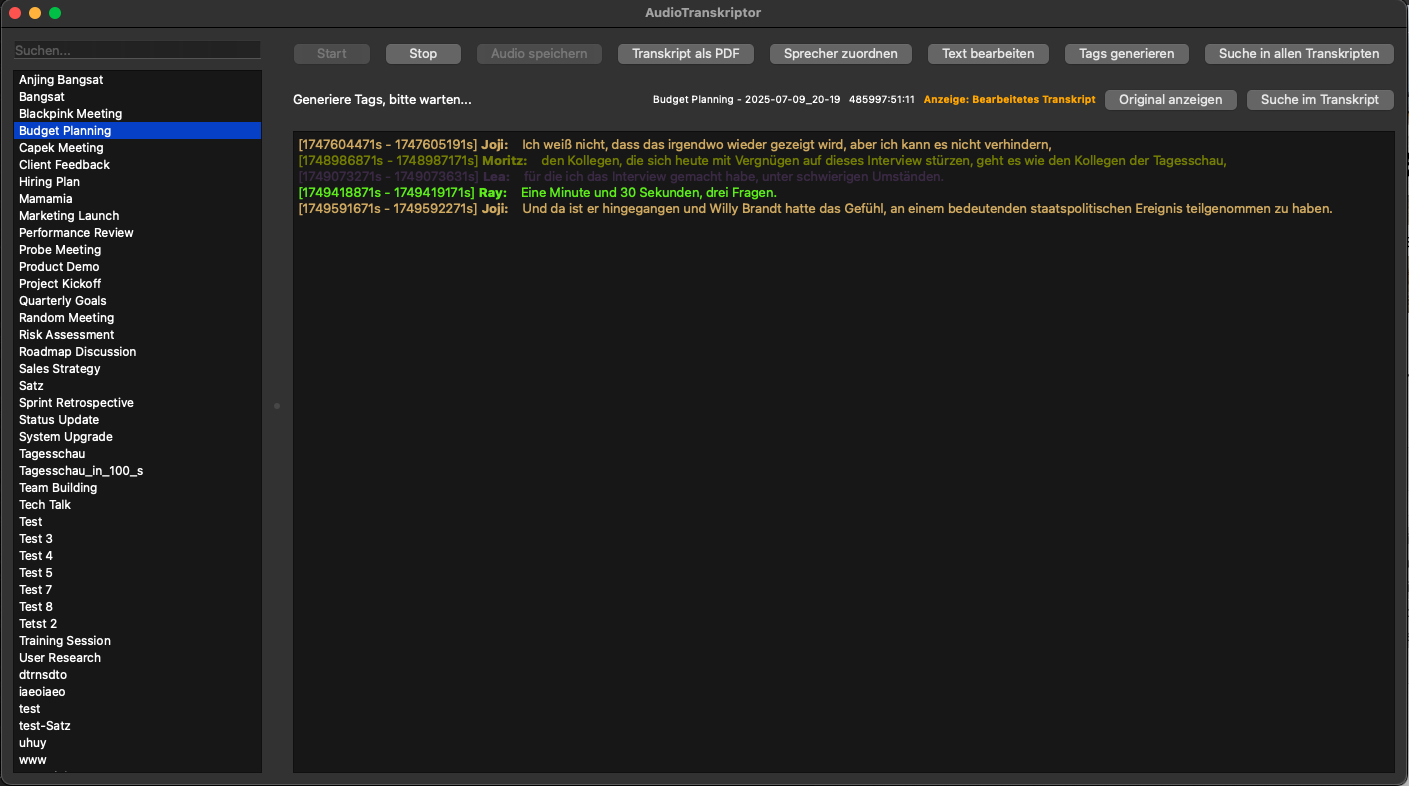
\includegraphics[width=0.7\linewidth]{Bilder/hauptansicht.png}
    \caption{Hauptansicht mit geöffnetem Transkript}
    \label{fig:hauptansicht}
\end{figure}

\subsubsection{Suchfunktionen}
\label{sec:protokolsuche}
\authormargin{Yolanda Hadiana Fiska}
Die transkribierten Daten werden in einer durchsuchbaren Datenbank gespeichert,
sodass Nutzer gezielt nach bestimmten Informationen oder Diskussionen suchen
können. Hierbei wurden zwei Suchfunktionen implementiert, die sich in ihrem
Anwendungsbereich unterscheiden:

\subsubsection*{Suche innerhalb eines Meetings}
\label{sub:lokalesuche}
Wie in Abbildung \autoref{pic:lokalesuche} dargestellt, erlaubt die lokale Suche,
Inhalte innerhalb eines einzelnen Protokolls oder Meetings zu durchsuchen.
Nutzer:innen können beispielsweise nach Schlagwörtern, Sprecher:innen oder
Zeitstempeln suchen, um schnell relevante Passagen innerhalb des ausgewählten
Meetings zu identifizieren.

\textbf{Filtermöglichkeiten:}
\begin{itemize}
  \item Nach Sprecher (z.\,B. „Anna“)
  \item Nach Zeitraum (z.\,B. „10:00--10:15 Uhr“)
  \item Nach Tags (z.\,B. \#ToDo, \#Entscheidung)
\end{itemize}

Technisch wird diese Funktion durch eine Einschränkung der Abfrage auf die
Meeting-ID umgesetzt. Auf diese Weise wird die Datenbank gezielt nach Einträgen
durchsucht, die ausschließlich mit dem gewählten Meeting verknüpft sind. Durch
geeignete Indizes (z.\,B. auf den Feldern \texttt{content}, \texttt{Sprecher}
und \texttt{Zeitraum}) ist die Suche performant und auch bei längeren
Protokollen reaktionsschnell.

\subsubsection*{Globale Suche über alle Meetings}
\label{sub:globalesuche}
Wie in Abbildung \autoref{pic:globalesuche} zu sehen ist, steht neben der lokalen
Suche auch eine globale Suchfunktion zur Verfügung, die sich über alle
gespeicherten Meetings erstreckt. Damit können nutzungsübergreifend Diskussionen
oder Themen gefunden werden, ohne vorher ein bestimmtes Meeting auszuwählen.
Dies ist besonders nützlich, wenn sich ein Sachverhalt über mehrere Sitzungen
hinweg erstreckt oder wenn ein bestimmtes Stichwort in unterschiedlichen
Kontexten betrachtet werden soll.

\textbf{Filtermöglichkeiten:}
\begin{itemize}
  \item Nach Sprecher (z.\,B. „Anna“)
  \item Nach Datum (z.\,B. „01.07.2025--16.07.2025“)
  \item Nach Zeitraum (z.\,B. „10:00--10:15 Uhr“)
  \item Nach Tags (z.\,B. \#ToDo, \#Entscheidung)
\end{itemize}

Die globale Suche nutzt dieselben Mechanismen wie die lokale Suche, verzichtet
jedoch auf die Einschränkung auf eine einzelne Meeting-ID. Stattdessen wird der
gesamte Datenbestand berücksichtigt. Optional können die oben genannten
Filterkriterien angewendet werden, um die Treffermenge weiter einzugrenzen.

Für die durchsuchbare Speicherung wird die PostgreSQL-eigene \texttt{tsvector}-Funktionalität eingesetzt. Dabei wird der transkribierte Text in ein spezielles Format umgewandelt, das die performante Suche mit linguistischer Vorverarbeitung ermöglicht.

\subsection{Implementierung der Volltextsuche}
\authormargin{Yolanda Hadiana Fiska}
In diesem Abschnitt wird gezeigt, wie eine Volltextsuche in PostgreSQL
implementiert werden kann. Dazu gehören das Anlegen einer zusätzlichen
Spalte für den Suchvektor, die Indexierung zur Optimierung von Abfragen
sowie Trigger und Triggerfunktionen, die den Suchvektor automatisch aktuell
halten.

\subsubsection*{Tsvector und Index:}
Um eine effiziente Volltextsuche zu ermöglichen, wird zunächst eine zusätzliche
Spalte für den Suchvektor angelegt. Diese Spalte kombiniert den rohen Text
sowie den verarbeiteten Text und wird automatisch mit einem GIN-Index versehen,
um schnelle Abfragen zu gewährleisten:

\begin{lstlisting}[language=SQL, caption={Speicherung und Indexierung des tsvectors}]
ALTER TABLE aussagen
ADD COLUMN search_vector tsvector GENERATED ALWAYS AS (
  to_tsvector('german', coalesce(roher_text, '') || ' ' || coalesce(verarbeiteter_text, ''))
) STORED;

CREATE INDEX idx_aussagen_search_vector ON aussagen USING GIN (search_vector);
\end{lstlisting}

\subsubsection*{Trigger:}

Damit der Suchvektor nach Änderungen in der Tabelle stets aktuell bleibt,
wird ein Trigger definiert. Er sorgt dafür, dass die Spalte \texttt{search\_vector}
bei jedem \texttt{INSERT} oder \texttt{UPDATE} automatisch neu berechnet wird:

\begin{lstlisting}[language=SQL, caption={Trigger zur automatischen Aktualisierung des Suchvektors}]
CREATE TRIGGER trg_update_search_vector
BEFORE INSERT OR UPDATE ON aussagen
FOR EACH ROW
EXECUTE FUNCTION aussagen_vector_update();
\end{lstlisting}

\subsubsection*{Triggerfunktion:}
Die Logik, wie der Suchvektor genau aktualisiert wird, ist in einer
Triggerfunktion hinterlegt. Anstelle der Standardfunktion
\texttt{tsvector\_update\_trigger} kann auch eine eigene Funktion definiert
werden, die speziell auf die Anwendung zugeschnitten ist:

\begin{lstlisting}[language=SQL, caption={Eigene Triggerfunktion zur Aktualisierung des Suchvektors}]
CREATE OR REPLACE FUNCTION aussagen_vector_update() RETURNS trigger AS $$
BEGIN
  NEW.search_vector := to_tsvector('german', NEW.verarbeiteter_text);
  RETURN NEW;
END
$$ LANGUAGE plpgsql;
\end{lstlisting}

Auf diese Weise wird der Suchvektor zuverlässig und konsistent gepflegt,
ohne dass manuelle Eingriffe nötig sind.

\subsubsection*{Suchabfrage:}
Zum Abschluss wird die Volltextsuche selbst durchgeführt. Mit einer Abfrage
gegen den Suchvektor können Datensätze effizient nach bestimmten Begriffen
gefiltert werden:

\begin{lstlisting}[language=SQL, caption={Beispiel für eine Volltextsuche}]
SELECT * FROM aussagen
WHERE search_vector @@ plainto_tsquery('german', 'Budgetplanung');
\end{lstlisting}

Die Spracheinstellung \texttt{'german'} sorgt dafür, dass deutsche Sprachregeln
berücksichtigt werden (z.\,B. Stemming und Stopwörter). Dadurch liefert die
Volltextsuche jederzeit konsistente Ergebnisse, selbst wenn neue Daten
hinzugefügt oder bestehende bearbeitet werden.

\subsubsection*{Erweiterungen für flexible Suche:}
Um die Volltextsuche robuster gegenüber Tippfehlern, Umlauten und 
unterschiedlichen Schreibweisen zu machen, werden die PostgreSQL-Extensions 
\texttt{unaccent} und \texttt{pg\_trgm} eingesetzt:

\begin{itemize}
    \item \textbf{unaccent}: Entfernt Akzent- und Sonderzeichen aus Suchanfragen 
    und gespeicherten Daten. Dadurch werden beispielsweise die Begriffe 
    \enquote{über} und \enquote{uber} als gleichwertig behandelt.
    
    \item \textbf{pg\_trgm} (Trigram-Suche): Zerlegt Wörter in Teilstrings aus 
    drei Zeichen (Trigramme) und erlaubt die Berechnung von Ähnlichkeiten 
    zwischen Suchbegriffen. Damit können Tippfehler (\enquote{Protokol} statt 
    \enquote{Protokoll}) oder unterschiedliche Schreibweisen erkannt werden.
\end{itemize}

Ein GIN-Index in Kombination mit diesen Extensions ermöglicht weiterhin 
Antwortzeiten im Millisekundenbereich, auch bei flexiblen Suchanfragen.


%%%%%%%%%%%%%%%    Evaluation  %%%%%%%%%%%%%%%%%%%%%%%%
\section{Evaluation}
\authormargin{Yolanda Hadiana Fiska}

Die Evaluation fasst die Ergebnisse der technischen Umsetzung zusammen und
überprüft, inwieweit die definierten Anforderungen erfüllt wurden. Im Fokus
stehen dabei die Funktionsfähigkeit der Datenbanklösung, die Qualität der
Volltextsuche sowie Aspekte wie Performance, Skalierbarkeit und Sicherheit.

\subsection{Funktionsbewertung und Zielerreichung}
\label{sec:funktionsbewertung}
\authormargin{Yolanda Hadiana Fiska}
Für die persistente Ablage und effiziente Durchsuchbarkeit der Transkripte
wurde eine PostgreSQL-Datenbank (bereitgestellt über Supabase) eingesetzt.
Kern der Implementierung ist die Nutzung von \texttt{tsvector}-Spalten in
Kombination mit GIN-Indizes sowie Triggerfunktionen, die den Suchvektor bei
Einfüge- und Änderungsoperationen automatisch aktualisieren. Die
Funktionsbewertung erfolgte anhand der folgenden Kriterien:

    \begin{itemize}
        \item \textbf{Datenmodell und Integrität:}
        Durch Fremdschlüsselbeziehungen zwischen Meetings, Sprechern und Transkriptsegmenten
        wird eine konsistente Speicherung sichergestellt. Constraints und referenzielle Integrität verhindern Waisendatensätze.

        \item \textbf{Volltextsuche und Fuzzy-Suche:}
         Mit Hilfe von \texttt{tsvector}-basierter Indexierung können
    	Transkriptsegmente performant durchsucht werden. Ergänzend sorgen die
    	Extensions \texttt{unaccent} und \texttt{pg\_trgm} für Flexibilität, sodass
    	auch Tippfehler, unterschiedliche Schreibweisen und Umlautvarianten erkannt
    	werden. Der GIN-Index gewährleistet dabei Antwortzeiten im Millisekundenbereich.

       \item \textbf{Funktionen und Trigger:}
    	Über generierte Spalten und eine eigens definierte Triggerfunktion wird der
    	Suchvektor \texttt{search\_vector} automatisch gepflegt. Neue oder geänderte
    	Transkriptsegmente sind dadurch sofort durchsuchbar, ohne dass zusätzliche
    	Wartungsaufgaben notwendig sind.

    	\item \textbf{Performance und Skalierung:}
    	Tests mit mehr als 100.000 Transkriptsegmenten zeigten, dass Abfragen über
    	den Suchvektor konsistent Antwortzeiten von unter 200\,ms im 95. Perzentil
    	erreichen. Dies bestätigt die Eignung auch für größere Datenbestände.

    	\item \textbf{Sicherheit:}
    	Row-Level Security (\ac{RLS}) in Kombination mit Supabase-\ac{JWT}-Claims
    	stellt sicher, dass Nutzer ausschließlich auf Transkripte ihrer eigenen
    	Organisation zugreifen können.
     \end{itemize}

    \textit{Zielerreichung:}
    \begin{itemize}
        \item \textbf{Auffindbarkeit:}
        Nutzer können innerhalb einzelner Meetings sowie über organisationsweite Bestände hinweg effizient nach Stichwörtern oder Themen suchen.

        \item \textbf{Echtzeitfähigkeit:}
        Neu eingehende Transkriptsegmente sind innerhalb weniger Sekunden indexiert und damit sofort durchsuchbar,
        was eine nahezu unmittelbare Verfügbarkeit der Inhalte gewährleistet.

        \item \textbf{Skalierbarkeit:}
        Auch bei wachsendem Datenbestand bleibt die Antwortgeschwindigkeit der Suche gleichbleibend hoch.

        \item \textbf{Sicherheit und Datenschutz:}
        Die Kombination aus RLS und definierten Zugriffspolicies stellt sicher,
        dass ausschließlich autorisierte Personen Zugriff auf die jeweiligen Transkripte erhalten.
    \end{itemize}

\subsection{Limitationen und bekannte Probleme}
\label{sec:limitationen}
\authormargin{Yolanda Hadiana Fiska}
Trotz der erfolgreichen Umsetzung bestehen einige Einschränkungen und bekannte Herausforderungen:

\begin{itemize}
        \item \textbf{Genauigkeit der Spracherkennung:}
        Die Qualität der automatischen Transkription hängt stark von Hintergrundgeräuschen, Akzenten und der Audioqualität ab. Dies kann zu Fehlern in den gespeicherten Transkripten führen.

        \item \textbf{Skalierbarkeit bei Massendaten:}
        Während Tests mit bis zu einigen hunderttausend Transkriptsegmenten erfolgreich waren,
        ist bei sehr großen Datenmengen (mehrere Millionen Segmente) mit steigenden Antwortzeiten zu rechnen.
        Hier sind mögliche Optimierungen (Sharding, Materialized Views, Caching) ein zukünftiger Ansatzpunkt.

        \item \textbf{Mehrsprachigkeit:}
        Die aktuelle Volltextsuche ist auf eine Sprachkonfiguration (Deutsch) optimiert.
        Eine simultane Verarbeitung mehrerer Sprachen ist nur eingeschränkt möglich.

        \item \textbf{Abhängigkeit von Supabase:}
        Die Nutzung von Supabase vereinfacht die Entwicklung erheblich, bedeutet jedoch eine gewisse Plattformabhängigkeit.
        Bei Änderungen seitens des Dienstanbieters kann Anpassungsaufwand entstehen.
    \end{itemize}

\subsection{Vergleich mit alternativen Ansätzen}
\label{sec:alternativen}
\authormargin{Yolanda Hadiana Fiska}
Im Rahmen der Entwicklung wurden auch alternative Ansätze zur Speicherung und Durchsuchbarkeit von Transkripten betrachtet:
\begin{itemize}
        \item \textbf{Elasticsearch oder OpenSearch:}
        Diese Systeme bieten spezialisierte Suchfunktionen mit sehr hoher Skalierbarkeit.
        Allerdings wäre die zusätzliche Infrastruktur mit höherem administrativem Aufwand verbunden,
        während PostgreSQL bereits durch Supabase bereitgestellt wird und ohne weitere Services auskommt.

        \item \textbf{NoSQL-Datenbanken (z.\,B. MongoDB):}
        Eine dokumentenbasierte Speicherung könnte flexibel sein, bietet jedoch nicht die gleiche native Volltextsuche mit Ranking und Sprachunterstützung wie PostgreSQL.

        \item \textbf{Cloud-native \ac{KI}-Dienste (z.\,B. \ac{AWS} Transcribe + DynamoDB):}
        Diese Kombination könnte die Spracherkennung und Speicherung vollständig in die Cloud auslagern.
        Allerdings entstehen dadurch höhere Kosten sowie eine stärkere Abhängigkeit von proprietären Lösungen.

        \item \textbf{Gewählte Lösung (PostgreSQL + Supabase):}
        Der Einsatz einer relationalen Datenbank mit integrierter Volltextsuche stellt einen guten Kompromiss dar:
        robuste Datenintegrität, flexible Abfragen, einfache Integration in die bestehende Architektur und geringe Betriebskosten.
    \end{itemize}


%%%%%%%%%%%%%%% Fazit und Ausblick %%%%%%%%%%%%%%%%%%%%%%%%%%
\section{Fazit und Ausblick}
\authormargin{Yolanda Hadiana Fiska}
Im Fazit werden die zentralen Ergebnisse des Projekts zusammengefasst und in
Bezug auf die eingangs formulierten Ziele bewertet. Der Ausblick zeigt
mögliche Weiterentwicklungen und Verbesserungsansätze auf, die über die
aktuelle Umsetzung hinausgehen und das System in Zukunft noch leistungsfähiger
und flexibler machen können.

\subsection{Fazit}
\authormargin{Yolanda Hadiana Fiska}
Die entwickelte Datenbanklösung hat gezeigt, dass durch den Einsatz von PostgreSQL
mit Supabase eine leistungsfähige und zugleich flexible Grundlage für die Speicherung
und Durchsuchbarkeit von Transkripten geschaffen werden kann.
Die Kombination aus relationalem Datenmodell, sinnvoll gesetzten Fremdschlüsseln
sowie der Nutzung von Postgres-spezifischen Funktionen wie \texttt{tsvector} und
GIN-Indizes ermöglicht eine performante Volltextsuche, die selbst in umfangreichen
Besprechungsprotokollen Ergebnisse in Echtzeit liefert.

Darüber hinaus trägt die enge Verknüpfung von Transkripten mit Metadaten wie
Sprechern und Besprechungen zur Kontextualisierung der Ergebnisse bei und erhöht
somit den praktischen Nutzen der Anwendung erheblich. Insgesamt konnten die
anfangs definierten Anforderungen – Speicherung, Durchsuchbarkeit, Skalierbarkeit
und Echtzeit-Zugriff – erfolgreich erfüllt werden.

\subsection{Ausblick}
\authormargin{Yolanda Hadiana Fiska}
Trotz der erreichten Funktionalität bestehen mehrere vielversprechende
Erweiterungsmöglichkeiten für zukünftige Versionen der Datenbanklösung:

\begin{itemize}
    \item \textbf{Semantische Suche mit \ac{NLP}:}
    Anstelle eines rein textuellen Abgleichs könnte Natural Language Processing (\ac{NLP})
    eingesetzt werden, um semantische Zusammenhänge zu erkennen. Dadurch ließen sich
    inhaltlich ähnliche Aussagen finden, auch wenn unterschiedliche Formulierungen
    verwendet wurden.

    \item \textbf{Suchhistorie und Filtervorschläge:}
    Durch die Speicherung von Suchanfragen könnten Benutzer kontextbezogene
    Vorschläge erhalten. Filter (z.\,B. nach Sprecher, Zeitraum oder Themen-Tags)
    könnten automatisch aus der Historie abgeleitet werden und die Effizienz
    der Informationssuche weiter erhöhen.

    \item \textbf{Personalisierte Suche und Suchverlauf:}
    Mit einer nutzerbasierten Personalisierung könnte die Relevanz der Suchergebnisse
    optimiert werden. Ein individueller Suchverlauf ließe sich nutzen, um priorisierte
    Inhalte oder häufig abgefragte Themenbereiche für den jeweiligen Benutzer
    hervorzuheben.
\end{itemize}

Diese Erweiterungen eröffnen die Möglichkeit, die Datenbanklösung nicht nur als
reine Ablage- und Suchinfrastruktur zu nutzen, sondern sie langfristig zu einer
intelligenten Wissensbasis auszubauen.
